\section{Introducción}

\begin{frame}{Introducción}
\begin{block}{Motivación}
La predicción del la vida útil remanente de un sistema mecánico disminuye el riesgo a fallas catastróficas y los costos de mantención. Ejemplo:
\begin{figure}
  \centering
  \subfloat{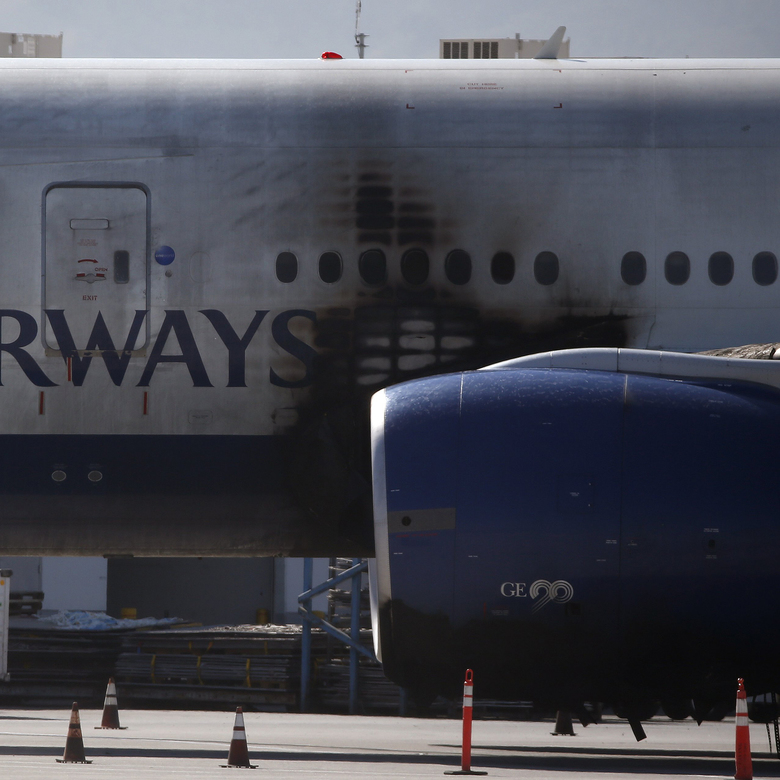
\includegraphics[scale=0.5]{animate/engine777.jpg}}\qquad
  \caption{Falla catastrófica avión 777, The Seattle Times. \cite{engine777}.}
  
\end{figure}
\end{block}
\end{frame}

\begin{frame}{Introducción}
\begin{block}{Motivación}
Falla catastrófica
\begin{figure}
  \centering
  \subfloat{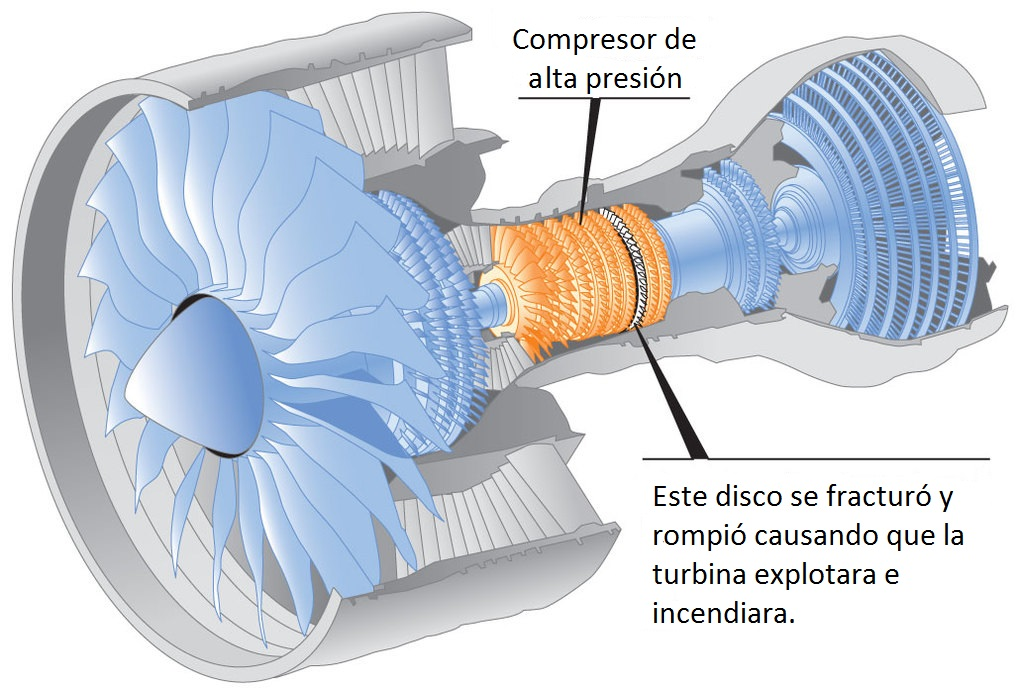
\includegraphics[scale=0.25]{animate/compressor-il-1020x688.jpg}}\qquad
  \caption{Falla catastrófica avión 777, The Seattle Times. (Imagen modificada \cite{engine777}).}
  
\end{figure}
\end{block}
\end{frame}



\begin{frame}{Introducción}

\begin{block}{Objetivo general}

Encontrar la mejor opción de red neuronal recurrente convolucional para la estimación de RUL en un sistema mecánico.
\end{block}
   
\end{frame}

\begin{frame}{Introducción}


\begin{block}{Objetivos específicos}

\begin{itemize}
    \item Estudiar modificación de la base de datos.
    \item Estudiar la aplicación de la Convolución en una serie de tiempo.
\end{itemize}
\end{block}
\end{frame}

\begin{frame}{Introducción}
\begin{block}{Alcances}
Programación y puesta en marcha de:


\begin{itemize}
    \item \textbf{ConvLSTM} 
    \item \textbf{ConvLSTM Codificadora-Decodificadora}
    \pause
    \item \textbf{ConvJANET} 
    \item \textbf{ConvJANET Codificadora-Decodificadora} 
\end{itemize}

\end{block}
   
\end{frame}